\documentclass[a4paper]{book}

\usepackage{geometry}
% make full use of A4 papers
\geometry{margin=1.5cm, vmargin={0pt,1cm}}
\setlength{\topmargin}{-1cm}
\setlength{\paperheight}{29.7cm}
\setlength{\textheight}{25.1cm}

% auto adjust the marginals
\usepackage{marginfix}

\usepackage{amsfonts}
\usepackage{amsmath}
\usepackage{amssymb}
\usepackage{amsthm}
%\usepackage{CJKutf8}   % for Chinese characters
\usepackage{ctex}
\usepackage{enumerate}
\usepackage{graphicx}  % for figures
\usepackage{layout}
\usepackage{multicol}  % multiple columns to reduce number of pages
\usepackage{mathrsfs}  
\usepackage{fancyhdr}
\usepackage{subfigure}
\usepackage{tcolorbox}
\usepackage{tikz-cd}
\usepackage{listings}
\usepackage{xcolor}
%------------------
% common commands %
%------------------
% differentiation
\newcommand{\gen}[1]{\left\langle #1 \right\rangle}
\newcommand{\dif}{\mathrm{d}}
\newcommand{\difPx}[1]{\frac{\partial #1}{\partial x}}
\newcommand{\difPy}[1]{\frac{\partial #1}{\partial y}}
\newcommand{\Dim}{\mathrm{D}}
\newcommand{\avg}[1]{\left\langle #1 \right\rangle}
\newcommand{\sgn}{\mathrm{sgn}}
\newcommand{\Span}{\mathrm{span}}
\newcommand{\dom}{\mathrm{dom}}
\newcommand{\Arity}{\mathrm{arity}}
\newcommand{\Int}{\mathrm{Int}}
\newcommand{\Ext}{\mathrm{Ext}}
\newcommand{\Cl}{\mathrm{Cl}}
\newcommand{\Fr}{\mathrm{Fr}}
% group is generated by
\newcommand{\grb}[1]{\left\langle #1 \right\rangle}
% rank
\newcommand{\rank}{\mathrm{rank}}
\newcommand{\Iden}{\mathrm{Id}}

% this environment is for solutions of examples and exercises
\newenvironment{solution}%
{\noindent\textbf{Solution.}}%
{\qedhere}
% the following command is for disabling environments
%  so that their contents do not show up in the pdf.
\makeatletter
\newcommand{\voidenvironment}[1]{%
  \expandafter\providecommand\csname env@#1@save@env\endcsname{}%
  \expandafter\providecommand\csname env@#1@process\endcsname{}%
  \@ifundefined{#1}{}{\RenewEnviron{#1}{}}%
}
\makeatother

%---------------------------------------------
% commands specifically for complex analysis %
%---------------------------------------------
% complex conjugate
\newcommand{\ccg}[1]{\overline{#1}}
% the imaginary unit
\newcommand{\ii}{\mathbf{i}}
%\newcommand{\ii}{\boldsymbol{i}}
% the real part
\newcommand{\Rez}{\mathrm{Re}\,}
% the imaginary part
\newcommand{\Imz}{\mathrm{Im}\,}
% punctured complex plane
\newcommand{\pcp}{\mathbb{C}^{\bullet}}
% the principle branch of the logarithm
\newcommand{\Log}{\mathrm{Log}}
% the principle value of a nonzero complex number
\newcommand{\Arg}{\mathrm{Arg}}
\newcommand{\Null}{\mathrm{null}}
\newcommand{\Range}{\mathrm{range}}
\newcommand{\Ker}{\mathrm{ker}}
\newcommand{\Iso}{\mathrm{Iso}}
\newcommand{\Aut}{\mathrm{Aut}}
\newcommand{\ord}{\mathrm{ord}}
\newcommand{\Res}{\mathrm{Res}}
%\newcommand{\GL2R}{\mathrm{GL}(2,\mathbb{R})}
\newcommand{\GL}{\mathrm{GL}}
\newcommand{\SL}{\mathrm{SL}}
\newcommand{\Dist}[2]{\left|{#1}-{#2}\right|}



%----------------------------------------
% theorem and theorem-like environments %
%----------------------------------------
\numberwithin{equation}{chapter}
\theoremstyle{definition}

\newtheorem{thm}{Theorem}[chapter]
\newtheorem{axm}[thm]{Axiom}
\newtheorem{alg}[thm]{Algorithm}
\newtheorem{asm}[thm]{Assumption}
\newtheorem{defn}[thm]{Definition}
\newtheorem{prop}[thm]{Proposition}
\newtheorem{rul}[thm]{Rule}
\newtheorem{coro}[thm]{Corollary}
\newtheorem{lem}[thm]{Lemma}
\newtheorem{exm}{Example}[chapter]
\newtheorem{rem}{Remark}[chapter]
\newtheorem{exc}[exm]{Exercise}
\newtheorem{frm}[thm]{Formula}
\newtheorem{ntn}{Notation}

% for complying with the convention in the textbook
\newtheorem{rmk}[thm]{Remark}


\lstset{
	breaklines,
	columns=fixed,       
	numbers=left,                                        % 在左侧显示行号
	numberstyle=\tiny\color{gray},                       % 设定行号格式
	frame=none,                                          % 不显示背景边框
	backgroundcolor=\color[RGB]{245,245,244},            % 设定背景颜色
	keywordstyle=\color[RGB]{40,40,255},                 % 设定关键字颜色
	numberstyle=\footnotesize\color{darkgray},           
	commentstyle=\it\color[RGB]{0,96,96},                % 设置代码注释的格式
	stringstyle=\rmfamily\slshape\color[RGB]{128,0,0},   % 设置字符串格式
	showstringspaces=false,                              % 不显示字符串中的空格
	language=c++,                                        % 设置语言
}
%----------------------
% the end of preamble %
%----------------------

\begin{document}
\pagestyle{empty}
\pagenumbering{roman}

\tableofcontents
\clearpage

\pagestyle{fancy}
\fancyhead{}
\lhead{Yan Tan}
\chead{booloperatordocument}
\rhead{\today}

\setcounter{chapter}{-1}
\pagenumbering{arabic}
% \setcounter{page}{0}

% --------------------------------------------------------
% uncomment the following to remove these environments 
%  to generate handouts for students.
% --------------------------------------------------------
% \begingroup
% \voidenvironment{rem}%
% \voidenvironment{proof}%
% \voidenvironment{solution}%


% each chapter is factored into a separate file.

\chapter{二维殷集程序实现文档}
% The main ingredients of snacks are sugar and fat;
%  the main ingredients of math are logic and set theory.
本篇文档是二维平面上的布尔运算的程序实现的设计文档。


%\begin{multicols%}{2}
%\setlength{\columnseprule}{0.2pt}  
\section{\heiti 作业题目}
实现张老师的论文《BOOLEAN ALGEBRA OF TWO-DIMENSIONAL CONTINUA
WITH ARBITRARILY COMPLEX TOPOLOGY》中定义的殷集和殷集集合
上的布尔运算。

\section{\heiti 数学定义}
\subsection{连通区域的边界 Jordan Curve}
Jordan Curve是首尾相连并且没有自相交的简单闭合曲线,详细见论文 \textbf{Theorem 3.5},
\textbf{Definition 3.6}和\textbf{Definition 3.7}.

\subsection{殷集边界 Spadjor}
Spadjor是Jordan Curve的集合,并且Jordan Curves之间包好关系可以
表示成哈斯图。详见论文 \textbf{Corollary 3.13., Corollary 3.14.}





\section{\heiti 数学概念的c++包装}

这个程序主体有5个类:

\subsection{点 class Point}
固有属性 :
\begin{itemize}
	\item  点的坐标 : coord[2] : double
	\item  每个点的唯一身份标识 : identity : int  (到Sweepline::points中O(1)的时间找出指定的点。)
	\item  是哪些线段的端点(以角度排序) : nearline : AVLTree<pair<double,  vector<int> > >(int唯一标识线段,double是这条线段与从此点开始的与x轴平行,方向是x轴正向的射线之间的逆时针方向的角度值) 
%	\item  容忍度 : tol : double
%	\item  static 成员,存储所有的点,与identity对应 : points : vector<Point>
\end{itemize}
固有操作 :
\begin{itemize}
	\item  读取修改点的坐标 : operator[](const int) : double
%	\item  求模 : norm() : double
	\item  计算相对位置 : operator-(const Point) : Point
	\item  判断是否同一个点 : operator==(const Point) : bool
	\item  判断两个点的大小顺序  : operator<(const Point) : bool, operator>(const Point) : bool 
	\item  点乘和叉乘用于计算有向面积大小  : dot(const Point) : double, cross(Point) : double
	\item  用于nearline中的线段按角度大小排序  : friend template<> operator<(const pair<double, vector<int> >,const pair<double, vector<int> >) : bool
	\item  输出与给定线段之间逆时针方向角度最小的线段  : nextline(const Line) : Line (要求给定线段必须以该点为端点)
	\item  添加,删除以此点为端点的线段在nearline中的记录 : addnearline(const Line) : void delnearline(const Line) : void
\end{itemize}

\subsection{线段 class Line}
固有属性 :
\begin{itemize}
	\item  线段的端点 : lp[2] : int   (到Sweepline::points中O(1)的时间找出指定点,方向为lp[0]->lp[1]。)
	\item  每条线的唯一身份标识  : identity : int  (Sweepline::lines中找出指定线段)
	\item  所在的jordanline  : injordanline  : int  (jordanlines中找出制定jordan线)
	\item  纵坐标较小的端点所在的x轴平行线l,l穿过的所有线段按交点x坐标大小排序orderline,orderline中该线段左边相邻的线段  : leftline  : int
	\item  lp[0]处该线段与x轴正向之间逆时针方向的角的弧度值[0, 2pi)  : angle : double
%	\item  容忍度  : tol : double
	\item  是否在另一个殷集内部  : IfInOtherYinset  : bool
%	\item  static 成员,存储所有线段  : lines  : vector<Line> 
\end{itemize}
固有操作 :
\begin{itemize}
	\item  输出端点 : operator[](const int) : Point
	\item  在确定y坐标时进行线段之间的比较,以交点的x轴坐标比较,使orderline中线段能进行排序 : operator<(const Line) : bool, operator>(const Line) : bool
%	\item  判断两条线是否在一条直线上 : coincide(const Line) : bool
	\item  计算点是否在另一个直线的上 : ifintheline(const Point) : int
	\item  判断两条线段是否相交 : ifintersection(const Line) : bool
	\item  计算两条线段所在直线的交点 : intersection(const Line) : Point
%	\item  判断两条线段是否有公共端点 : connect(const Line) : bool
	\item  输出角度 : angle() : double
	\item  输出在哪条jordan线内 : injordanline() : int
	\item  输出是否在另一个殷集内 : IfInOtherYinset() : bool
	\item  static 函数从已有line集合lines内生成Jordanlines并更新相应数据 : generator() : vector<Jordanline>
\end{itemize}
\subsection{Jordan线 class Jordanline}
固有属性 :
\begin{itemize}
	\item  包含的线段 : line : vector<int>  (到Sweepline::lines中查找)
	\item  身份标识 : identity : int 
	\item  以这个Jordan线的最左下的端点为终点的在这个Jordan线内的线段 : leftmostline : int
	\item  从最左下端点出发向左的射线第一个相交的Jordan线 : leftJordanline : int
	\item  内边界或者外边界,即方向顺时针或逆时针,type当jl是外边界时为1,内边界时为0 : type : int
%	\item  static 成员, 存储所有Jordanline : jordanlines : vector<Jordanline>
\end{itemize}
固有操作 :
\begin{itemize}
	\item  返回身份标识 : identity() : int
	\item  更新leftmostline,leftjordanline等数据,为generator()生成Spajor提供数据 : update() : void
	\item  static 函数从已有的Jordan线集合Jordanlines生成Spajor : generator() : Spajor 
\end{itemize}
\subsection{Spajor 与殷集一一对应 class Spajor}
固有属性 :
\begin{itemize}
	\item  殷集的边界集合,是一组Jordan线 : jordanline : vector<int> (到Jordanline的static成员jordanlines中取出相应的Jordan线集合)
	\item  树结构的哈斯图,表现jordanline中的jordan线的包含关系 :hassmap : HassNode* 
	\item  Spajor的类型,若无穷远处属于它,type为true,否则为false : type : bool
	\item  身份标识 : identity : int
\end{itemize}
固有操作 :
\begin{itemize}
	\item  布尔运算求补 : complement() : Spajor
	\item  布尔运算求交 : meet(const Spajor) : Spajor
	\item  布尔运算求并 : join(const Spajor) : Spajor
	\item  输出输入数据,依次输出Jordan线,按线段的方向依次输出点的坐标 : friend operator<<(ostream\&, Spajor) : ostream\&  friend operator>>(istream\&, Spajor)
\end{itemize}
\subsection{哈斯图存储结构 HassNode}
固有属性 :
\begin{itemize}
	\item  身份标识 : identity : int
	\item  父节点 : int
	\item  子节点 : vector<int> 
\end{itemize}
\subsection{数据存储结构平衡二叉树  template<class T> class AVLTree}
固有属性 :
\begin{itemize}
	\item  \begin{itemize}
		\item  树节点结构 template<class T> class AVLTreeNode
		\item  数据  : data : T
		\item  深度  : height : int
		\item  左,右,父节点 : Left, Right, father : AVLTreeNode<T>*
	\end{itemize}
    \item  根节点  : Root : AVLTreeNode<T>*
\end{itemize}
固有操作 :
\begin{itemize}
	\item  加入数据  : add(T) : AVLTreeNode<T>*
	\item  可以删除指针指定的树节点或数据。 : del(T) : bool; del(AVLTreeNode<T>*) : bool
	\item  查找某个数据和查找前一个或后一个数据  : find(T) : AVLTreeNode<T>*, 
	findprevnode(AVLTreeNode<T>*) : AVLTreeNode<T>*, findnextnode(AVLTreeNode<T>*) : AVLTreeNode<T>*
	\item  查找第一个数据和最后一个数据  : findfirstnode() : AVLTreeNode<T>*, 
	findlastnode() : AVLTreeNode<T>*
\end{itemize}
\subsection{扫描线  class sweepline}
固有属性 :
\begin{itemize}
	\item  static成员,水平扫描线的y轴坐标,用于线段排序。  y : double
	\item  static成员,用平衡二叉树存储扫描线法的事件点  eventpoint : AVLTree<Point>
	\item  static成员,用平衡二叉树存储扫描线法过程中的有序线段  orderline, orderline2, orderline3  : AVLTree<Line>
	\item  static成员,扫描线算法,存储每条线在orderline,orderline2,orderline3中的树节点指针  
	orderlinemark, orderlinemark2, orderlinemark3 : AVLTree<pair<int, AVLTreeNode<Line>*>> 
	\item  static成员,存储所有点。 points : vector<Point>
	\item  static成员,存储所有线。 lines : vecotr<Line>
	\item  static成员,存储所有还在图上的点和线的identity。 existpoints : AVLTree<int> ; existlines : AVLTree<int>;
	\item  static成员,存储所有Jordanline。 jordanlines : vector<Jordanline>
	\item  static成员,存储所有还在图形上的Jordanline的identity。 existjordanlines : vector<int>
	\item  static成员,存储所有Spajor。  spajors : vector<Spajor>
\end{itemize}
固有操作:
\begin{itemize}
	\item  static函数,扫描线法计算所有交点,和更新Line::leftline,Line::IfInOtherYinset。
	intersection() : void
	\item  static函数, 在扫描算法中用来计算两条线是否有交点,若有,更新eventpoint,lines等数据。 : inter(Line) : void
\end{itemize}
%\label{sec:logic}
%\input{sec/logic.tex}

\section{\heiti  类之间的关系,UML类图}
之前的类互相依赖,继承关系如图1所示
\begin{itemize}
	\item  \begin{math}
		\dashleftarrow
	\end{math} 虚线箭头是依赖关系,即类的实现需要箭头指向的另一个类的协助
	\item  \begin{math}
		\lozenge-
	\end{math}空心菱形直线是聚合关系,即菱形所指的类是另一个类的组合。
	\item  \begin{math}
		\blacklozenge-
	\end{math}实心菱形直线是组合关系,和聚合的区别是部分不能单独存在。
\end{itemize}

\begin{figure}
	\centering
	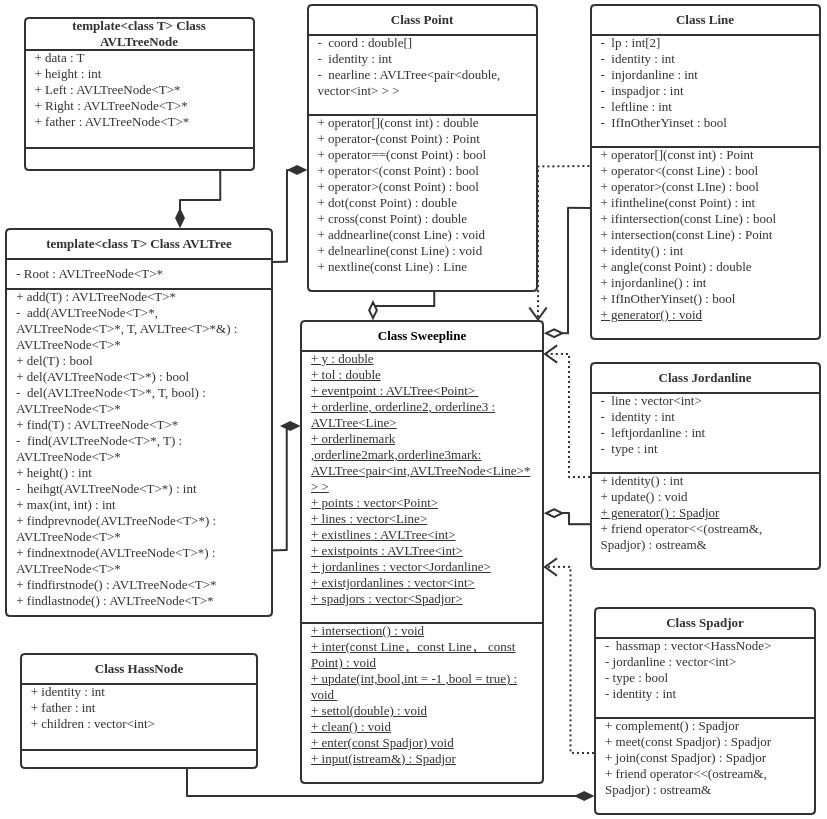
\includegraphics[width=\textwidth]{UMLboolean.png}
    \caption{以上所有类的关系的UML图}
\end{figure}
%\label{sec:sets}
%\input{sec/orderedSets.tex}

\section{\heiti 算法设计与证明}

\subsection{Point}

\subsubsection{Point::operator[](const int)}
\paragraph{契约}
\subparagraph{input}
输入一个int和一个Point类;
\subparagraph{output}
输出一个double或者Point类的坐标引用用于修改坐标,通过重载函数实现,具体调用取决于需要;
\subparagraph{precondition}
输入的int是0或1,Point类已经初始化;
\subparagraph{postcondition}
对应于int的值为0或1,分别输出这个Point的x轴坐标和y轴坐标。
\paragraph{算法实现}
直接输出输入的Point类的成员coord[i]的右值或左值。
\paragraph{证明}
直接可得正确性。

\subsubsection{Point::norm()}
\paragraph{契约}
\subparagraph{input}
输入一个表示向量的Point类p。
\subparagraph{output}
输出double值。
\subparagraph{precondition}
输入的Point类已经初始化。
\subparagraph{postcondition}
输出的double值是输入的Point到0点之间的距离,也是表示的向量的长度,结合operator-可以计算点之间的距离。
\paragraph{算法实现}
\begin{lstlisting}
	double d0 = coord[0], d1 = coord[1];
	return squrt(d1 * d1 + d2 * d2);
\end{lstlisting}
\paragraph{证明}
由距离和模长的定义,算法符合要求。

\subsubsection{Point::operator-(const Point)}
\paragraph{契约}
\subparagraph{input}
输入两个Point类p1,p2。
\subparagraph{output}
输出一个表示两个点相对位置的Point类,也是表示p1到p2的向量的Point类。
\subparagraph{precondition}
输入的类p1,p2已初始化。
\subparagraph{postcondition}
输出的点,x,y轴坐标分别等于p1的x,y轴坐标减p2的x,y轴坐标.
\paragraph{算法实现}
\begin{lstlisting}
	return Point(coord[0] - p2.coord[0], coord[1] - p2.coord[1]);
\end{lstlisting}
\paragraph{证明}
x,y轴坐标减法计算得到输出的点的横纵坐标,之后调用构造函数。

Sbo\subsubsection{Point::operator<(const Point)}
\paragraph{契约}
\subparagraph{input}
输入两个Point类p1,p2。
\subparagraph{output}
输出一个bool值。
\subparagraph{precondition}
输入的类片,p2已初始化。
\subparagraph{postcondition}
a和b在容忍度为tol的情况下的字典排序比大小结果。即a的y轴坐标比b的y轴坐标小tol,或者当a的y轴坐标-b的y轴坐标绝对值小于tol时,a的x轴坐标比b的x轴坐标小tol,这两种情况返回true,其他情况返回false。
\paragraph{算法实现}
\begin{lstlisting}
	if(coord[1] < p2.coord[1] - tol){
		return true;
	}
	else if((coord[1] > p2.coord[1] - tol) && (coord[1] < p2.coord[1] + tol) ){
		if(coord[0] < p2.coord[0] - tol){
		return true;
		}
	}
	return false;
\end{lstlisting}
\paragraph{证明}
由字典排序定义,符合要求。
\subsubsection{Point::operator>(const Point)}
契约与operator<()类似,输出结果相反。因此
交换参数顺序,调用operator<(),返回小于操作符返回的bool值。

\subsubsection{Point::dot(const Point)}
\paragraph{契约}
\subparagraph{input}
输入两个Point类p1,p2。
\subparagraph{output}
输出double值
\subparagraph{precondition}
输入的p1,p2要是operator-()输出的表示向量的Point类。
\subparagraph{postcondition}
输出的double值是两个向量的点乘结果。
\paragraph{算法实现}
\begin{lstlisting}
	return (coord[0] * p2.coord[0] + coord[1] * p2.coord[1]);
\end{lstlisting}
\paragraph{证明}
正确性由点乘定义得。

\subsubsection{Point::cross(const Point)}
\paragraph{契约}
\subparagraph{input}
输入两个Point类p1,p2。
\subparagraph{output}
输出double值
\subparagraph{precondition}
输入的p1,p2要是operator-()输出的表示向量的Point类。
\subparagraph{postcondition}
输出的double值是两个向量的叉乘结果。
\paragraph{算法实现}
\begin{lstlisting}
return (coord[0] * p2.coord[1] - coord[1] * p2.coord[0]);
\end{lstlisting}
\paragraph{证明}
正确性由叉乘定义得

\subsubsection{friend template<> operator<(const pair<double, int>,const pair<double,int>)}
用于Point类的以此点为端点的线段集合nearline排序,double是Line与x轴正向之间的逆时针方向角的弧度值angle,int是Line类的身份标识identity。
\paragraph{契约}
\subparagraph{input}
输入两个Pair<double,int> pa1,pa2。
\subparagraph{output}
输出bool值。
\subparagraph{precondition}
仅用于泛型算法sort()将nearline排序中。
\subparagraph{postcondition}
输出按double值的大小比较结果。由于是double值比较,这里设置的容忍度是tol/100.
\paragraph{算法实现}
\begin{lstlisting}
	if(pa1.first < pa2.first - tol/100) return true;
	else return false;
\end{lstlisting}
\paragraph{证明}
由实现显然。

\subsubsection{Point::nextline(const Line)}
输入Line l2在已排序的nearline成员中查找,Line l1,使得(l2 - l1)在mod(2π)意义下最小。
\paragraph{契约}
\subparagraph{input}
输入一个Line类l2和一个nearline  vector<pair<double,vector<int>>>。
\subparagraph{output}
输出一个Line类l1,不会在nearline中删除l1,l2。
\subparagraph{precondition}
l2必须在nearline集合中。由每次调用nearline的点是l2的终点来保证。要求nearline中在容忍度tol/100的情况下有相等的弧度,并且没有存储在一个vector<int>内。nearline必须已排序。这个点的出度等于入度。
\subparagraph{postcondition}
输出的Line类l1的起点p是输入的l2的终点。并且它们之间不存在以p点为起点的Line类l使得$\angle l2 \rightarrow l < \angle l2 \rightarrow l1$。
\paragraph{算法实现}
\begin{lstlisting}
    Line Point::nextline(const Line& l2){
    bool t = false, t1 = false;
    Line l1;
    vector<int> l2v;
    l2v.push_back(l2.identity());
    AVLTreeNode<pair<double, vector<int>>* k = nearline.find(make_pair(l2.angle(), l2v));
    if(k == NULL) cout << "nextline() k out of range";
	k = nearline.findprevnode(k);
	if(k == NULL) k = nearline.findlastnode();
	if(k != NULL){
	    for(auto i = 0; i < k->data.second.size(); i++){
	    if(t == true && t1 == false){
			    if(k->data.second[i][0] == identity){
				    t1 = true;
				    l1 = lines[k->data.second[i]];
			    }
		    }
		    if(k->data.second[i] == l2.identity()){
			   	t = true;
		    }
	    }
    }
    if(t1 != true){
	    k = nearline.find(make_pair(l2.angle(), l2v));
	    if(k != NULL){
		    for(auto i = 0; i < k->data.second.size(); i++){
		    	if(t == true && t1 == false){
			    	if(k->data.second[i][0] == identity){
				    	t1 = true;
				   		l1 = lines[k->data.second[i]];
			   		}
				}
				if(t == false && k->data.second[i] == l2.identity()){
			    t = true;
				}
		    }
	    }
    }
    bool test = false;
    while(t1 != true){
	    k = nearline.findnextnode(k);
	    if(k == NULL){
		    k = nearline.findfirstnode();
		    if(test == false)
		    	test = true;
		    else {
		    	cout << "nextnearline() wrong test";
		    	exit(0);
		    }
		}
		if(k != NULL){
		    for(auto i = 0; i < k->data.second.size(); i++){
			    if(t == true && t1 == false){
				    if(k->data.second[i][0] == identity){
					    t1 = true;
					    l1 = lines[k->data.second[i]];
				    }
			    }
			    if(t == false && k->data.second[i] == l2.identity()){
			    	t = true;
			    }
		    }
	    }
	    if(t1 == true) break;
    }
    return l1;
    }
\end{lstlisting}
\paragraph{证明}
nearline是按double值排序,几乎重合的线段存储在一个double和angle的差小于tol/100的pair<double, vector<int> >中的vector中。因此首先按l2的angle值搜索必会搜索到l2所在的pair pa1。若pa1中的vector有以l2的终点p为起点的线段l1,那么l1闭符合条件,因为$\angle l2 \rightarrow l1 = 0$,不会有更小的逆时针角。若pa1的vector中没有符合要求的l1,那么按angle值继续往前搜索,若指针是nearline的第一个则将指针移到最后一点。由出度等于入度,必将搜索到符合要求的l1。

\subsubsection{Point::addnearline(const Line)}
\paragraph{契约}
\subparagraph{input}
输入一个Line类l,和一个Point类p的nearline。
\subparagraph{output}
在p的nearline中添加l.identity。
\subparagraph{precondition}
p是l的端点之一。
\subparagraph{postcondition}
若nearline中已有pair的double数据与l.angle的差小于tol/100。则将l.identity加入到这个pair的vector<int>中。其余情况插入一个新pair<double l.angle, vector<int> lv(l.identiy())>。
\paragraph{算法实现}
\begin{lstlisting}
	vector<int> lv;
	lv.push_back(l.identity());
	pair<double, vector<int> pa = make_pair(l.angle(), lv);
	AVLTreeNode<pair<double, vector<int>>>* k = nearline.find(pa);
	if(k == NULL)
		nearline.add(pa);
	else
		k->data.second.insert(l.identity());
	
\end{lstlisting}
\paragraph{证明}
首先构造一个pair,使用AVLTree的接口函数find()在nearline中搜寻是否已有pair满足double值足够接近。如果有,find()返回这个pair,将l的身份标识identity插入到pair的第二项vector中。如果没有,find()返回NULL,将以l的数据生成的pair插入到nearline中。

\subsubsection{Point::delnearline(const Line)}
\paragraph{契约}
\subparagraph{input}
输入一个Line类l,和一个Point类p的nearline。
\subparagraph{output}
在p的nearline中删除l.identity。
\subparagraph{precondition}
p是l的端点,并且l的nearline中有保存l.identity。
\subparagraph{postcondition}
删除nealine中保存的l.identity。若此时存在pair的vector为空,将存储这个pair的节点从AVLTree中删除。
\paragraph{算法实现}
\begin{lstlisting}
	void Point::delnearline(const Line& l2){
		bool t = false;
		vector<int> l2v;
		l2v.push_back(l2.identity());
		AVLTreeNode<pair<double, vector<int>>* k = nearline.find(make_pair(l2.angle(), l2v));
		if(k == NULL) cout << "nextline() k out of range";
		k = nearline.findprevnode(k);
		if(k == NULL) k = nearline.findlastnode();
		if(k != NULL){
			auto i = k->data.second.begin();
			while(i != k->data.second.end()){
				if(t == false && (*i) == l2.identity()){
					t = true;
					if (k->data.second.size() == 1){
						nearline.del(k);
						break;
					}
					else{
						k->data.second.erase(i);
						break;
					}
				}
				i++;
			}
		}
		else cout << "delnearline() wrong";
		if(t != true){
			k = nearline.find(make_pair(l2.angle(), l2v));
			if(k != NULL){
				auto i = k->data.second.begin();
				while(i != k->data.second.end()){
					if(t == false && (*i) == l2.identity()){
						t = true;
						if(k->data.second.size() == 1){
							nearline.del(k);
							break;
						}
						else{
							k->data.second.erase(i);
							break;
						}
					}
					i++;
				}
			}
		}
		bool test = false;
		while(t != true){
			k = nearline.findnextnode(k);
			if(k == NULL){
				k = nearline.findfirstnode();
				if(test == false)
					test = true;
				else {
					cout << "nextnearline() wrong test";
					exit(0);
				}
			}
			if(k != NULL){
				auto i = k->data.second.begin();
				while(i != k->data.second.end()){
					if(t == false && (*i) == l2.identity()){
						t = true;
						if(k->data.second.size() == 1){
							nearline.del(k);
							break;
						}
						else{
							k->data.second.erase(i);
							break;
						}
					}
					i++;
				}
			}
			if(t1 == true) break;
		}
	}
\end{lstlisting}
\paragraph{证明}
由l的数据构造一个pair,使用find()在nearline中搜索充分接近的double值的pair。l只可能存储在搜索到的节点的前一个或者后一个,只有这3个节点的pair.first的double值可能与l.angle值的差小于tol/100,因为每个pair.first值的差大于tol/100。在搜索到的vector中,如果只有一个值直接删除,还有其他值时只删除l.identity。

\subsection{Line}
\subsubsection{Line::operator[](const int)}
\paragraph{契约}
\subparagraph{input}
输入Line l,int i,point集合Sweepline::points。
\subparagraph{output}
输出point p。
\subsubsection{precondition}
i等于0或1。l已经初始化。
\subsubsection{postcondition}
i等于0时输出l的起点,i等于1时输出终点。
\paragraph{算法实现}
\begin{lstlisting}
	return Sweepline::points[l.lp[i]];
\end{lstlisting}
\paragraph{证明}
访问类数据成员借助static成员Sweepline::points输出需要的点。

\subsubsection{Line::operator<(const Line)}
用于在扫描线上对线段排序
\paragraph{契约}
\subparagraph{input}
输入两个Line l1,ll2;一个扫描线y轴坐标double sweepline::y;
\subparagraph{output}
输出bool值反映大小关系
\subparagraph{precondition}
l1,l2与y轴坐标为sweepline::y的x轴平行线l有交点,
%并且l1,l2的两个端点坐标y轴坐标差小于tol时即非常接近(即有l1[1].[1] - l1[0].[1] < tol => l1[1].[1] - l1[0].[1] < tol/1000)。
\subparagraph{postcondition}
输出l1和l2与扫描线l的交点的x轴坐标的大小比较。
\paragraph{算法实现}
\begin{lstlisting}
	vector<Point>& points = Sweepline::points;
	vector<Line>& lines = Sweepline::lines;
	Line l1 = lines[this->identity]; 
	Line l2 = lines[ll2.identity()];
	l1 = lines[l1.identity()];
	double y = sweepline::y;
	double x1 = min(min(points[l1[0]].[0],points[l1[1]].[0]), min(points[l2[0]].[0],points[l2[1]].[0]));
	double x2 = max(max(points[l1[0]].[0],points[l1[1]].[0]), max(points[l2[0]].[0],points[l2[1]].[0]));
	Point a1(x1, y), a2(x2, y);
	Line l3(a1, a2);
	Point p1, p2;
	Point l1p0 = points[l1[0]], l1p1 = points[l1[1]], l2p0 = points[l2[0]], l2p1 = points[l2[1]];
	if(l1p0 > l1p1) { l1p0 = points[l1[1]]; l1p1 = points[l1[0]];}
	if(l2p0 > l2p1) { l2p0 = points[l2[1]]; l2p1 = points[l2[0]];}
	if(l3.ifintheline(l1p1)) p1 = l1p1;
	if(l3.ifintheline(l1p0)) p1 = l1p0;
	if(l3.ifintheline(l2p1)) p2 = l2p1;
	if(l3.ifintheline(l2p0)) p2 = l2p0;
	if(l3.ifintheline(l1p1) == false && l3.ifintheline(l1p0) == false) 
		p1 = l1.intersection(l3);
	if(l3.ifintheline(l2p1) == false && l3.ifintheline(l2p0) == false) 
		p2 = l2.intersection(l3);
	return p1[0] < p2[0];
	
\end{lstlisting}
\paragraph{证明}
先判断l1与扫描线是否重合coincide,若重合输出左端点。不重合调用intersection()计算交点。最后通过判断交点的顺序可得扫描线与线段相交的顺序,因为重合时左端点即是第一次相交。

\subsubsection{Line::operator>(const Line)}
交换参数顺序之后,调用operator<(),输出<输出的bool值。

\subsubsection{Line::ifintheline(const Point)}
\paragraph{契约}
\subparagraph{input}
输入Line l,Point p,double tol,Sweepline::points。
\subparagraph{output}
输出bool值。
\subparagraph{precondition}
l,p已初始化。
\subparagraph{postcondition}
若在容忍度tol下,与p点调用Point::operator==返回true的所有点都不在l上时返回0,否则返回1。
\paragraph{算法实现}
\begin{lstlisting}
	Point lp1 = Sweepline::points[l[0]], lp2 = Sweepline::points[l[1]];
	if(p == lp1 || p == lp2) reutrn 1;
	if((p[0] < min(lp1[0],lp2[0]) - Sweepline::tol) || (p[0] > max(lp1[0],lp2[0]) + Sweepline::tol)
	 ||(p[1] < min(lp1[1],lp2[1]) - tol) || (p[1] > max(lp1[0],lp2[1]) + tol))
		return 0;
	Point p1 = Point(p[0] - tol, p[1] - tol);
	Point p2 = Point(p[0] + tol, p[1] - tol);
	Point p3 = Point(p[0] - tol, p[1] + tol);
	Point p4 = Point(p[0] + tol, p[1] + tol);
	if(((p1 - lp1).cross(lp1 - lp2) * (p - lp1).cross(lp1 - lp2)) > 0 &&
	   ((p2 - lp1).cross(lp1 - lp2) * (p - lp1).cross(lp1 - lp2)) > 0 &&
	   ((p3 - lp1).cross(lp1 - lp2) * (p - lp1).cross(lp1 - lp2)) > 0 &&
	   ((p4 - lp1).cross(lp1 - lp2) * (p - lp1).cross(lp1 - lp2)) > 0)
	   return 0;
	 return 1;
\end{lstlisting}
\paragraph{证明}
首先判断p是否与l的端点充分接近,然后判断p是否在线段l附近。再将与p点在容忍度tol的情况下等价的所有点所在的正方形的四个顶点p1,p2,p3,p4取出,若正方形内存在点在l所在直线上,那么这四个顶点也必然在l所在直线的两边或者上面。对任一顶点都计算p1和l两个顶点之间的有向面积乘p和l两个顶点的有向面积,如果是正数说明在同一边,为0说明有一点在l所在直线上,为负数说明在两边。又因为前面已经判断p在l附近,结合得l是否包含与p等价的点。

\subsubsection{Line::coincide(const Line)}
\paragraph{契约}
\subparagraph{input}
输入Line l1,l2。
\subparagraph{output}
输出 int值
\subparagraph{precondition}
l1,l2已初始化。
\subparagraph{postcondition}
判断l1,l2是否重合,即l1,l2上的两个端点是同一个点。
\paragraph{算法实现}
\begin{lstlisting}
	if(l1[0] == l2[0] || l1[0] == l2[1]){
		if(l1[1] == l2[0] || l1[1] == l2[1])
			return 1;
	}
	return 0;
	
\end{lstlisting}

	
\paragraph{证明}
直接比较Line类中存储的端点身份标识进行比较是否是同一个点。如果都是返回1,否则返回0。

\subsubsection{Line::ifintersection(const Line)}
\paragraph{契约}
\subparagraph{input}
输入Line l1,l2。
\subparagraph{output}
输出bool值。
\subparagraph{precondition}
l1,l2已初始化。l1的端点不在l2上,l2端点不在l1上。
\subparagraph{postcondition}
输出l1,l2是否有交点,若有输出true,没有输出false。
\paragraph{算法实现}
\begin{lstlisting}
	vector<Point>& points = Sweepline::points
	Point p10 = points[l1[0]], p11 = points[l1[1]],p20 = points[l2[0]], p21 = points[l2[1]];
	if(((p10 - p20).cross(p20 - p21)) * ((p11 - p20).cross(p20 - p21)) < 0 &&
	   ((p20 - p10).cross(p10 - p11)) * ((p21 - p10).cross(p10 - p11)) < 0)
		return true;
	return false;  
\end{lstlisting}
\paragraph{证明}
同上计算有向面积,两条线段相交等价于一条线段的两个端点分别在另一条线段的所在直线的两端,并且由于没有一条线段端点在另一条线段上,所以它们必交与内部。
\subsubsection{Line::intersection(const Line)}
\paragraph{契约}
\subparagraph{input}
输入两条Line l1,l2。
\subparagraph{output}
输出一个Point p。
\subparagraph{precondition}
l1,l2有内部交点,线段端点不在另一条线段上,l1,l2不重合。
\subparagraph{postcondition}
输出的Point是l1,l2的内部交点,在容忍度tol下交点和端点不等价。
\paragraph{算法实现}
\begin{lstlisting}
	vector<Point>& points = Sweepline::points
	Point p1 = points[l1[0]], p2 = points[l1[1]],p3 = points[l2[0]], p4 = points[l2[1]];
	double s1 = fabs((p1 - p2).cross(p2 - p3)), s2 = fabs((p1 - p2).cross(p2 - p4)));
	return Point((p4[0] * s1 + p3[0] * s2)/(s1 + s2), (p4[1] * s1 + p3[1] * s2)/(s1 + s2));
\end{lstlisting}
\paragraph{证明}
计算$\triangle p1p2p3$和$\triangle p1p2p4$的面积,面积的比值等于交点到线段端点的距离比值,所以交点的坐标可以通过面积的比值和端点坐标算出。

\subsubsection{Line::angle(const Point)}
\paragraph{契约}
\subparagraph{input}
Line l,Point p。Sweepline::points。
\subparagraph{output}
double
\subparagraph{precondition}
l已初始化,p是l的端点,points中存储了它的端点。
\subparagraph{postcondition}
输出与在起点为p的x轴正向射线之间的弧度值。范围[0 - $\varepsilon$,2PI - $\varepsilon$)。$\varepsilon$是tol导致的。
\paragraph{算法实现}
\begin{lstlisting}
	Point p0,p1;
	if(l.lp[0] == p.identity()) { p0 = points[lp[0]]; p1 = points[lp[1]];}
	else { p1 = points[lp[0]]; p0 = points[lp[1]];}
	Point p = p1 - p0;
	double d;
	if(p[0] > 0) {
		d = atan(p[1]/p[0]);
		if(d < 0) d = d + 2 * PI;
	}
	else if(p[0] < 0) {
		d = atan(-p[1]/p[0]); d = PI - d;
	}
	else {
		if(p[1] > 0) d = PI / 2;
		else if(p[1] < 0) d = PI * 3 / 2;
		else exit(0);
	}
	return d;  
\end{lstlisting}
\paragraph{证明}


\subsubsection {Line类中还有一些访问和修改私有成员:identity,leftline,IfinOtherYinset的成员函数,例如identity()和setidentity()等。}
\paragraph{契约}
\subparagraph{input}
输入一个Line l。
\subparagraph{output}
输出私有成员的数据或数据引用。
\subparagraph{precondition}
l已初始化。
\subparagraph{postcondition}
根据需要输出数据或数据的引用。
\paragraph{算法实现}
\begin{lstlisting}
	return identity;
\end{lstlisting}
\paragraph{证明}

\subsubsection{static Line::generator()}
\paragraph{契约}
\subparagraph{input}
Line类集合Sweepline::lines,Point集合Sweepline::points。现存所有Line类的identity集合Sweepline::existlines
\subparagraph{output}
更新Sweepline::jordanlines的数据。
\subparagraph{precondition}
Sweepline::lines内的每个Line l的端点Point的nearline集合已全部更新,并且出度等于入度。
\subparagraph{postcondition}
输出的是还没有更新leftjordanline,leftmostline,type默认值的Jordanline类集合vector<vector<Jordanline>。
\paragraph{算法实现}
\begin{lstlisting}
	void Line::generator() {
		vector<Point> points = Sweepline::points;
		vector<Line>& lines = Sweepline::lines;
		AVLTree<int> existl = Sweepline::existlines;
		vector<Jordanline>& jordanlines = Sweepline::jordanlines;
		AVLTree<int>& existjordanlines = Sweepline::existjordanlines
		vector<int> jordanline;
		int l, p, k;
		int k = Sweepline::jordanlines.size();
		AVLTree<pair<int, int>> jvl;
		while(true){
			if(existl.findfirstnode() == NULL) break;
			l = (existl.findfirstnode())->data;
			p = l[0];
			jvl.push_back(make_pair(p, l));
			while(true){
				int l1 = l;
				int p2 = lines[l1][1];
				int l2 = (points[p2].nextline(lines[l1]).identity());
				p = p2;
				l = l2;
				while(jvl.find(make_pair(p, l)) != NULL){
					int pp1 = (jvl.find(make_pair(p, l))->data).first;
					int ll1 = (jvl.find(make_pair(p, l))->data).second;
					int pp2 = lines[ll1][1];
					p = pp2;
					if(p == p2){
						points[pp1].delnearline(ll1);
						points[pp2].delnearline(ll2);
						jvl.del(make_pair(pp1, ll1));
						existl.del(ll1);
						lines[ll1].setinjordanline(k);
						jordanline.add(ll1);
						Jordanline jordan(jordanline, k);
						jordanlines.push_back(jordan);
						jordanline.erase(jordanline.begin, jordanline.end());
						existjordanlines.push_back(k);
						k++;
						break;
					}
					int ll2 = (points[pp1].nextline(lines[ll1])).identity();
					points[pp1].delnearline(ll1);
					points[pp2].delnearline(ll1);
					jvl.del(make_pair(pp1, ll1));
					existl.del(ll1);
					lines[ll1].setinjordanline(k);
					jordanline.add(ll1);
					l == ll2;
				}
				if(jvl.empty()) break;
				p = p2;
				l = l2;
				jvl.add(make_pair(p, l));
			}
		}
	}
	
\end{lstlisting}
\paragraph{证明}
首先由每个点出度等于入度,由定理2.12知可以生成一些圈恰好遍历所有边。又因为遍历时寻找nextline时取逆时针角最小的边,结合不存在Point类以外的交点,可得产生的圈没有不合适的交点。还有算法中的遍历的路径上若出现重复的点,将重复的点之间的路径截下产生一个新的圈,因此每个圈不会出现自相交。综上产生的圈都是jordan线的vector集合。

\subsection{Jordanline}
\subsubsection{Jordanline的私有数据:identity,leftjordanline,type的更新函数Jordanline::update()}
\paragraph{契约}
\subparagraph{input}
输入Jordanline jl,和jl.vector<int>中对应的Sweepline::lines中的Line类。
\subparagraph{output}
更新jl.leftjordanline,jl.leftmostline,jl.type。
\subparagraph{precondition}
图上所有的line类已经划分到一个个Jordanline类中而且更新了leftline和injordanline数据,vector<int>中代指的线段是按jordan线的方向依次排列的。
\subparagraph{postcondition}
更新后的leftmostline是jl以最左下角的点为终点的边的identity,leftjordanline是jl最左下角的Point出发的向左射线第一个相交的Line所在的Jordanline的identity。type当jl是外边界时输出1,内边界时输出0。
\paragraph{算法实现}
\begin{lstlisting}
	vector<Line>& lines = Sweepline::lines;
	vector<Point>& points = Sweepline::points;
	Point p = lines[line[0]].[1];int j = 0;
	for(auto i = 1; i < line.size(); i++){
		if(lines[line[i]].[1] < p) {p = lines[line[i]].[1]; j = i;}
	}
	leftmostline = j;
	if(lines[line[j]].leftline() == -1) leftjordanline = -1;
	else {
		leftjordanline = lines[lines[line[j]].leftline()].injordanline();
		if(leftjordanline == identity && lines[line[j + 1]].leftline() != -1) 
		leftjordanline = lines[lines[line[j + 1]].leftline()].injordanline();
		else leftjordanline = -1;
	}
	Point p1 = points[lines[line[j]].[0]],p2 = points[lines[line[j]].[1]],p3 = points[lines[line[j + 1]].[1]];
	if((p1 - p2).cross(p2 - p3) < 0) type = 0;
	else { type = 1;}
\end{lstlisting}
\paragraph{证明}
首先在jl的边集合中按顺序遍历找到最左下的Point p,设置leftmostline为以这条线段为终点的Line l。由于p是字典排序最小的点,所以从p出发的向左的射线相交的顺序可以在扫描线算法中orderline的线段顺序得到记录在l.leftline中,除了与左边的jordan线相交,有可能先与jl中另一条以p为端点的边交于点p,所以先判断一次是否等于identity如过等于,取另一条边的leftline才是左下的jordan线上的边。因为p是最左下点,顺时针或逆时针直接通过计算与p相邻的三个点组成依jl的方向的顺序围成的三角形的有向面积的正负性可得。
\subsubsection{static Jordanline::generator()}
\paragraph{契约}
\subparagraph{input}
输入所有Jordanline的集合jordanlines。
\subparagraph{output}
输出一个Spajor。
\subparagraph{precondition}
jordanlines内的所有Jordanline jl都已经调用update()更新过数据。
\subparagraph{postcondition}
输出的Spajor能一一对应到殷集,殷集的边界Jordan线集合由jordanlines确定,需要在Spajor中完成哈斯图体现jordan线之间的包含关系。
\paragraph{算法实现}
\begin{lstlisting}
	vector<int> existjordanlines = Sweepline::existjordanlines;
	AVLTree<pair<int,int>> mark;
	vector<Jordanline>& jordanlines = Sweepline::jordanlines; 
	vector<Spajor>& spajors = Sweepline::spajors;
	Jordanline jl;
	vector<HassNode> vhn(existjordanlines.size() + 1);
	for(int i = 0; i < existjordanlines.size() + 1; i++){
		int j = existjordanlines[i];
		mark.add(make_pair(existjordanlines[i],i));
		HassNode hn(j);
		vhn.push_back(hn);
	}
	HassNode hn(existjordanlines.size());
	vhn.push_back(hn);
	for(int i = 0; i < existjordanlines.size(); i++){
		jl = jordanlines[existjordanlines[i]];
		while(jl.type == (jordanlines[existjordanlines[i]].type())){
			if(jl.leftjordanline == -1) break;
			jl = jordanlines[jl.leftjordanline];
		}
		if(jl.leftjordanline == -1) { 
			vhn[i].father = existjordanlines.size();
			vhn[existjordanlines.size()].children.push_back(i);
		}
		else { 
			int j = mark.find(make_pair(jl.identity(),0)).second;
			vhn[i].father = j;
			vhn[j].children.push_back(i);
		}
	}
	int k = spajors.size();
	jl = jordanlines[vhn[*(vhn.end()--).children[0]].identity];
	bool b;
	if(jl.type == 1) b = false;
	else b = true;
	return Spajor(vhn, existjordanlines, b, k);
\end{lstlisting}
\paragraph{证明}
主要是更新jordan线的包含关系,定义最后一个hassnode对应无穷远处依情况定方向的Jordan线。对每一个jordan线l,因为每次调用leftjordanline转移到下一个Jordan曲线都会使得左下点在字典排序上更小所以不会循环,又因为Jordan线数量有限。所以要么是找到合适的和l方向相反的jordan线l2包含l,此时更新l对应的hassnode的father为l2的identity,并且添加l.identity到l2对应的hassnode的children中。要么不存在l2符合要求,则更新l对应的hassnode的father为无穷远处jordan线,并且加入到最后一个hassnode的children中添加l.identity。由于每个hassnode(除了无穷远处jordan线对应的hassnode)只有唯一的子父关系对应于被包含关系,并且每个hassnode都会更新一次father,所以Spajor所有的包含关系都保存到hassnode中了。

\subsection{Spajor}
\subsubsection{Spajor::complement()}
\paragraph{契约}
\subparagraph{input}
输入Sparjor。Sweepline::points,Sweepline::lines,Sweepline::jordanlines。
\subparagraph{output}
输出Sparjor。更新Sweepline::points,Sweepline::lines,Sweepline::jordanlines。
\subparagraph{precondition}
输入的Sparjor是殷集A。A的边界Line和Point都以经存储在Sweepline::points,Sweepline::lines中。
\subparagraph{postcondition}
输出的Sparjor表示的是A的补集。
\paragraph{算法实现}
\begin{lstlisting}
	vector<Line>& lines = Sweepline::lines;
	for(auto i = 0; i < jordanline.size(); i++){
		Jordanline jl = jordanline[i];
		int j = jl.size();
		vector<int> jl1(j);
		for(auto i = 0; i < jl.size(); i++){
			jl1[j - i - 1] = jl[i];
			int m = lines[jl[i]].[0];
			lines[jl[i]].[0] = lines[jl[i]].[1];
			lines[jl[i]].[1] = j;
		}
	}
\end{lstlisting}
\paragraph{证明}
首先调换A边界上所有lines中存储的所有线段的方向,即遍历所有边并交换端点顺序。其次,还要调换殷集边界的边的存储顺序,因为jordan线是按线段方向存储的,所以要随着边的变向一起变向。通过对Sweeplines::jordanlines中所有Jordanline::line中的Line类identity的顺序换向,同时改变这些边的方向。

\subsubsection{Spajor::meet(Spajor)}
\paragraph{契约}
\subparagraph{input}
输入两个Spajor A和B。Sweepline::points,Sweepline::lines,Sweepline::jordanlines。
\subparagraph{output}
输出一个Spajor C,并更新Sweepline::points,Sweepline::lines,Sweepline::jordanlines中的Point类,Line类和Jordanline类的数据。
\subparagraph{precondition}
A和B的边界上的Point类,Line类和Jordanline类都已经初始化并输入到Sweepline::points,Sweepline::lines,Sweepline::jordanlines中。
\subparagraph{postcondition}
C是A,B的交,Sweepline::points添加新的交点,Sweepline::lines添加新的线段(不删除原有线段,只是删除所有调用方式,比如Point::nearline和原来的Jordanline类),Sweepline::jordanlines删除原有的Jordanline输入新的Jordanline(因为原有的jordan线已经不是Jordan线了)。
\paragraph{算法实现}
\begin{lstlisting}
	调用Sweepline::intersection()计算所有交点并更新points和lines内类的数据(例如Point::nearline,Line::leftline,Line::angle)。
	遍历lines中所有Line l,若l.IfInOtherYinset为false将l.lp[]对应的Point p 中删除p.nearline中代表l的数据,当IfInOtherYinset为true时跳过。
	调用Line::generator()生成新的vector<Jordanline> 替换原jordanlines。
	遍历jordanlines中所有Jordanline类分别调用Jordanline::update()更新内部数据。
	调用Jordanline::gennerator()生成一个Spajor类C,输出C。
\end{lstlisting}
\paragraph{证明}
	intersection()算出了所有交点,并将新产生的有向线段都插入到lines中。因此A和B中所有边还在lines中或被划分为多条Line(原Line的Point中的访问路径已被删除约等于懒惰删除,只保留了可能是C的边的所有Line类)。
	
	遍历并利用IfInOtherYinset筛选边,由于Line l属于C的边当且仅当l.IfInOtherYinset为true,所以删除所有false的边的Point中的访问路径后,当且仅当Line l是C的边界时才能从Point中访问l。
	
	Line::generator()从现存的Line中生成一组只更新了Jordanline::line的Jordanline类的vector<Jordanline>,每个Jordanline类代表一个jordan线而且两两之间没有不合适的交点。因此这组jordan线就是C的边界集合。
	
	最后生成Spajor还需要jordan线之间的包含关系,因此从line中的leftline信息调用Jordanline::update()更新leftjordanline数据。调用Jordanline::generator()生成唯一的Spajor由Spajor和Jordanline的一一对应关系知所得的Spajor即是C。
	
\subsubsection{Spajor::join(Spajor)}
\paragraph{契约}
\subparagraph{input}
同 meet();
\subparagraph{output}
同 meet();
\subparagraph{precondition}
同 meet();
\subparagraph{postcondition}
C是A和B的交
\paragraph{算法实现}
\begin{lstlisting}
	调用A.complement(),B.complement;
	调用C = A.meet(B);
	调用C.complement();
	输出C。
\end{lstlisting}
\paragraph{证明}
	由布尔运算的交并补关系得。
	
\subsubsection{friend operator<<(ostream\&, Spajor)}
\paragraph{契约}
\subparagraph{input}
Spajor C。
\subparagraph{output}
点坐标输入到ostream中。
\subparagraph{precondition}
C是Jordanline::generator()生成的。
\subparagraph{postcondition}
首先输出Spajor::jordanline.size(),再依次输出C边界上的jordan线,即jordanline中存储的Jordanline类。输出Jordanline类时先输出Jordanline::line.size()再依次输出line中的Line类。输出line类时只输出起点Point的坐标。
\paragraph{算法实现}
\begin{lstlisting}
	for(auto i = 0; i < jordanline.size(); i++){
		Jordanline jl = jordanlines[i];
		os << jl;
	}
\end{lstlisting}
\paragraph{证明}
依次调用符合条件的重载operator<<操作符。

\subsubsection{friend operator>>(istream\&, Spajor)}
\paragraph{契约}
\subparagraph{input}
首先输入读入殷集Y边界的Jordan线的数量,然后以Jordan线的方向依次读入jordan线上的点。
\subparagraph{output}
Spajor类,lines,points,jordanlines中加入新的类。
\subparagraph{precondition}
输入的数据是一组jordan线上按jordan线方向输入的点的坐标,这些jordan线是Y的所有边界。
\subparagraph{postcondition}
输出的Spajor内的hassmap体现了所有jordan线的包含关系,jordanline是Y的所有jordan线边界的identity的集合。
\paragraph{算法实现}
\begin{lstlisting}
	int i;
	is >> i;
	vector<int> jordanline(i);
	int k = 0;
	while(k < i){
		生成Point,Line,Jordanline并插入到Sweepline::points,Sweepline::lines,Sweepline::jordanlines中。
		k++;
	}
\end{lstlisting}
\paragraph{证明}

\subsection{Sweepline}
\subsubsection{Sweepline::intersection()}
\paragraph{契约}
\subparagraph{input}
vector<Point> points,vector<Line> lines,AVLTree<Point> eventpoint, AVLTree<Line> orderline1,orderline2,orderline3 ,AVLTree<int> existlines,AVLTree<int> existpoints。
\subparagraph{output}
vector<Point> points,vector<Line> lines, AVLTree<int> existlines, AVLTree<int> existpoints。
\subparagraph{precondition}
eventpoint,orderline1,orderline2,orderline3都为空,existlines和existpoints存储所有还存在于图上的Line和Point。points,lines存储所有从程序开始就产生的Point和Line。
\subparagraph{postcondition}
计算出所有的交点,构造Point并插入到points中。交点划分线段,在existlines中删除被划分的Line l0.identity并插入新的两个Line l1.identity, l2.identity。交点中nearline,加入l1 l2,原来的线段端点的nearline都删除l0,分别插入l1或l2。若出现两个点充分接近,合并成字典排序中较小的点,并且合并nearline,更新nearline中所有线段的端点,从existpoints中删除被合并的Point的identity。
\paragraph{算法实现}
\begin{lstlisting}
	for(auto i = 0; i < existpoints.size(); i++){
		eventpoint.add(points[existpoints[i]]);
	}
	AVLTreeNode<Line>* orderlinemarkp;
	AVLTreeNode<Line>* prev = NULL,next = NULL;
	AVLTreeNode<Point>* atnp = eventpoint.findfirstnode();
	while(true){
		prev = NULL;
		next = NULL;
		Point p = atnp->data;
		y = p[1];
		AVLTree<Point>* m = eventpoint.findnextnode(atnp),mt = NULL;
		while(m->data == p){
			Point q = m->data;
			AVLTree<pair<double,vector<int> >* z = q.nearline.findfirstnode();
			while(z != NULL){
				vector<int> vi = ((z->data).second;
				for(auto k = 0; k < vi.size(); k++){
					if(lines[vi[k]].[0] == q.identity()) 
						lines[vi[k]].[0] = p.identity();
					if(lines[vi[k]].[1] == q.identity()) 
						lines[vi[k]].[1] = p.identity();
					points[p.identity()].addnearline(lines[vi[k]]); 
				}
				z = q.nearline.findnextnode(z);	
			}
			mt = m;
			existpoints.del(q.identity());
			m = eventpoint.findnextnode(m);
			eventpoint.del(mt->data);
		} 
		AVLTree<pair<double,vector<int>>* atndv = p.nearline.findfirstnode();
		while(true){
			vector<int> v = (atndv->data).second;
			for(auto i = 0; i < v.size(); i++){
				Line l = lines[v[i]];
				if(points[l[0]] < p || points[l[1]] < p){
					if(orderlinemark.find(make_pair(l.identity(), NULL)) == NULL) cout << "orderlinemark wrong\n";
					orderlinemarkp = orderlinemark.find(make_pair(l.identity(),NULL))->data.second;
					prev = orderline.findprevnode(orderlinemarkp);
					next = orderline.findnextnode(orderlinemarkp);
					orderline.del(orderlinemarkp);
					orderlinemark.del(make_pair(l.identity(),orderlinemarkp));
				}
			}	
			atndv = p.nearline.findnextnode(atndv);	
			if(atndv == NULL) break;
			if((atndv->data).first < PI + tol/100) break;	
		}
		if(atndv != NULL){
			vector<int> v = (atndv->data).second;
			Line l = lines[v[0]];
			if(prev == NULL && next == NULL){
				orderlinemarkp = orderline.add(l);
				prev = orderline.findprevnode(orderlinemarkp);
				next = orderline.findnextnode(orderlinemarkp);
				orderline.del(orderlinemarkp);
			}
		}
		while(next != NULL && (next->data).ifintheline(p)){
			Line nextline = lines[(next->data).identity()];
			existlines.del(nextline.identity());
			orderline.del(orderlinemark.find(make_pair(nextline.identity(),NULL))->data.second);
			orderlinemark.del(make_pair(nextline.identity(),NULL));
			int k = lines.size();
			Line l1(nextline[0], p.identity(), k, nextline.inspajor());
			lines.push_back(l1);
			k++;
			Line l2(p.identity(), nextline[1], k, nextline.inspajor());
			lines.push_back(l2);
			points[p.identity()].addnearline(l1);
			points[p.identity()].addnearline(l2);
			points[nextline[0]].delnearline(nextline);
			points[nextline[0]].addnearline(l1);
			points[nextline[1]].delnearline(nextline);
			points[nextline[1]].addnearline(l2);
			next = orderline.findnextnode(next);
		}
		while(prev != NULL || (prev->data).ifintheline(p)){
			Line prevline = lines[(prev->data).identity()];
			existlines.del((prevline.identity());
			orderline.del(orderlinemark.find(make_pair(prevline.identity(),NULL))->data.second);
			orderlinemark.del(make_pair(prevline.identity(),NULL));
			int k = lines.size();
			Line l1(prevline[0], p.identity(), k, prevline.inspajor());
			lines.push_back(l1);
			k++;
			Line l2(p.identity(), prevline[1], k, prevline.inspajor());
			lines.push_back(l2);
			points[p.identity()].addnearline(l1);
			points[p.identity()].addnearline(l2);
			points[prevline[0]].delnearline(prevline);
			points[prevline[0]].addnearline(l1);
			points[prevline[1]].delnearline(prevline);
			points[prevline[1]].addnearline(l2);
			prev = orderline.findprevnode(prev);
		}
		atndv = p.nearline.findfirstnode();
		Line leftl,rightl;
		int g = 0;
		Line l;
		while(true){
			vector<int> v = (atndv->data).second;
			for(auto i = 0; i < v.size(); i++){
				l = lines[v[i]];
				if(points[l[0]] > p || points[l[1]] > p){
					if(g == 0){ leftl = l; g = 1;}
					orderlinemarkp = orderline.add(l);
					orderlinemark.add(make_pair(l.identity(),orderlinemarkp));
				}
			}	
			atndv = p.nearline.findnextnode(atndv);	
			if(atndv == NULL) {rightl = l;break;}		
		}			
		if(g == 1){
			if(prev != NULL) inter(prev->data,leftl,p);
			if(next != NULL) inter(rightl,next->data,p);
		}
		else {
			if(prev != NULL && next != NULL) 
			inter(prev->data,next->data,p);
		}
		atnp = eventpoint.findnextnode(atnp);
		if(atnp == NULL) break;
	}
\end{lstlisting}
\paragraph{证明}

\subsubsection{Sweepline::inter()}
\paragraph{契约}
\subparagraph{input}
输入两个Line l1 l2 和当前eventpoint p1判断交点是否已处理。
\subparagraph{output}
根据l1,l2是否相交,更新eventpoint ,orderline,lines,points,existpoints,existlines内Point.nearline和Line::lp的数据等
\subparagraph{precondition}
Line l1,l2初始化并已在lines,existlines等集合中。
\subparagraph{postcondition}
若没有交点无变化,若有交点,更新相应的信息。
\paragraph{算法实现}
\begin{lstlisting}
	AVLTreeNode<Line>* orderlinemarkp;
	Line prevl = lines[l1.identity()], l = lines[l2.identity()];
	Point lp0,lp1,prevlp0,prevlp1;
	if(points[l[0]] < points[l[1]]) {
		lp0 = points[l[0]];lp1 = points[l[1]];
	}
	else {
		lp0 = points[l[1]];lp1 = points[l[0]];
	}
	if(points[prevl[0]] < points[prevl[1]]) {
		prevlp0 = points[prevl[0]];prevlp1 = points[prevl[1]];
	}
	else {
		prevlp0 = points[prevl[1]];prevlp1 = points[prevl[0]];
	}
	if(lp0 == prevlp0){
		AVLTree<pair<double,vector<int> >* z = lp0.nearline.findfirstnode();
		while(z != NULL){
			vector<int> vi = ((z->data).second;
			for(auto k = 0; k < vi.size(); k++){
				if(lines[vi[k]].[0] == lp0.identity()) 
				lines[vi[k]].[0] = prevl0.identity();
				if(lines[vi[k]].[1] == lp0.identity()) 
				lines[vi[k]].[1] = prevl0.identity();
				points[prevlp0.identity()].addnearline(lines[vi[k]]); 
			}
			z = lp0.nearline.findnextnode(z);	
		}
		existpoints.del(lp0.identity());
		eventpoint.del(lp0);
	}
	else if(prevl.ifintheline(lp0)){
		int k = lines.size();
		Line l1(prevl[0], lp0.identity(), k, prevl.inspajor());
		lines.push_back(l1);
		k++;
		Line l2(lp0.identity(), prevl[1], k, prevl.inspajor());
		lines.push_back(l2);
		existlines.del(prevl.identity());
		existlines.add(l1.identity());
		existlines.add(l2.identity());
		orderlinemarkp = orderlinemark.find(make_pair(prevl.identity(),NULL))->data.second;
		if(prevl[0] < lp0) { 
			orderlinemarkp->data = l1;
			orderlinemark.del(make_pair(prevl.identity(),NULL));
			orderlinemark.add(make_pair(l1.identity(),orderlinemarkp));
		}
		else {
			orderlinemarkp->data = l2;
			orderlinemark.del(make_pair(prevl.identity(),NULL));
			orderlinemark.add(make_pair(l2.identity(),orderlinemarkp));
		}
		points[lp0.identity()].addnearline(l1);
		points[lp0.identity()].addnearline(l2);
		points[prevl[0]].delnearline(prevl);
		points[prevl[0]].addnearline(l1);
		points[prevl[1]].delnearline(prevl);
		points[prevl[1]].addnearline(l2)
	}
	else if(l.ifintheline(prevlp0)){
		int k = lines.size();
		Line l1(l[0], prevlp0.identity(), k, l.inspajor());
		lines.push_back(l1);
		k++;
		Line l2(prevlp0.identity(), l[1], k, l.inspajor());
		lines.push_back(l2);
		existlines.del(l.identity());
		existlines.add(l1.identity());
		existlines.add(l2.identity());
		orderlinemarkp = orderlinemark.find(make_pair(l.identity(),NULL))->data.second;
		if(l[0] < prevlp0) { 
			orderlinemarkp->data = l1;
			orderlinemark.del(make_pair(l.identity(),NULL));
			orderlinemark.add(make_pair(l1.identity(),orderlinemarkp));
		}
		else {
			orderlinemarkp->data = l2;
			orderlinemark.del(make_pair(l.identity(),NULL));
			orderlinemark.add(make_pair(l2.identity(),orderlinemarkp));
		}
		points[prevlp0.identity()].addnearline(l1);
		points[prevlp0.identity()].addnearline(l2);
		points[l[0]].delnearline(l);
		points[l[0]].addnearline(l1);
		points[l[1]].delnearline(l);
		points[l[1]].addnearline(l2);
	}
	else {
		if(l.ifintersection(prevl)) {
			Point p = prevl.intersectoin(l);
			if(p < p1) return;
			int k = points.size();
			p.setidentity(k);
			points.push_back(p);
			existpoints.add(k);
			k = lines.size();
			Line l1(p.identity(), prevl[1], k, prevl.inspajor());k++;
			Line l2(prevl[0], p.identity(), k, prevl.inspajor());k++;
			Line l3(l[0], p.identity(), k, l.inspajor());k++;
			Line l4(p.identity(), l[1], k, l.inspajor());
			lines.push_back(l1);lines.push_back(l2);lines.push_back(l3);lines.push_back(l4);
			existlines.del(prevl.identity());
			existlines.del(l.identity());
			existlines.add(l1.identity());
			existlines.add(l2.identity());
			existlines.add(l3.identity());
			existliens.add(l4.identity());
			points[p.identity()].addnearline(l1);
			points[p.identity()].addnearline(l2);
			points[p.identity()].addnearline(l3);
			points[p.identity()].addnearline(l4);
			eventpoint.add(points[p.identity()]);
			orderlinemarkp = orderlinemark.find(make_pair(prevl.identity(),NULL))->data.second;
			orderlinemark.del(make_pair(prevl.identity(),NULL));
			if(p > prevl[1]) {
				orderlinemarkp->data = l1;
				orderlinemark.add(make_pair(l1.identity(),orderlinemarkp));
			}
			else {
				orderlinemarkp->data = l2;
				orderlinemark.add(make_pair(l2.identity(),orderlinemarkp));
			} 
			orderlinemarkp = orderlinemark.find(make_pair(l.identity(),NULL))->data.second;
			orderlinemark.del(make_pair(l.identity(),NULL));
			if(p > l[0]) {
				orderlinemarkp->data = l3;
				orderlinemark.add(make_pair(l3.identity(),orderlinemarkp));
			}	
			else {
				orderlinemarkp->data = l4;
				orderlinemark.add(make_pair(l4.identity(),orderlinemarkp));
			}
			points[l[0].identity()].delnearline(l);
			points[l[0].identity()].addnearline(l3);
			points[l[1].identity()].delnearline(l);
			points[l[1].identity()].addnearline(l4);
			points[prevl[0].identity()].delnearline(prevl);
			points[prevl[0].identity()].addnearline(l2);
			points[prevl[1].identity()].delnearline(prevl);
			points[prevl[1].identity()].addnearline(l1);
		}
	}
\end{lstlisting}
\paragraph{证明}

\subsubsection{Sweepline::update(int, bool, int = -1, bool = true)}
\paragraph{契约}
\subparagraph{input}
输入lines,points等。算两个交点的Spajor::identity int spajor2,spajor3,和type,spajortype2,spajortype3。还有一个标记m,是meet或complement决定是否更新IfInOtherYinset。
\subparagraph{output}
更新lines中Line的Line::leftline,Line::IfInOtherYinset。
\subparagraph{precondition}
intersection()函数调用后调用。
\subparagraph{postcondition}
设置leftline为线段下节点是在orderline中前一个Line的identity。IfInOtherYinset设置为它是否在另一个殷集内部。
\paragraph{算法实现}
\begin{lstlisting}
	for(auto i = 0; i < existpoints.size(); i++){
		eventpoint.add(points[existpoints[i]]);
	}
	int m = 0;
	if(spajor3 != -1) m = 1;
	AVLTreeNode<Line>* orderlinemarkp;
	AVLTreeNode<Line>* prev = NULL;
	AVLTreeNode<Point>* atnp = eventpoint.findfirstnode();
	while(true){
		AVLTree<pair<double,vector<int>>* atndv = p.nearline.findfirstnode();
		while(true){
			vector<int> v = (atndv->data).second;
			for(auto i = 0; i < v.size(); i++){
				Line l = lines[v[i]];
				if(points[l[0]] < p || points[l[1]] < p){
					if(orderlinemark.find(make_pair(l.identity(), NULL)) == NULL) cout << "orderlinemark wrong\n";
					orderlinemarkp = orderlinemark.find(make_pair(l.identity(),NULL))->data.second;
					prev = orderline.findprevnode(orderlinemarkp);
					if(prev != NULL) lines[l.identity()].setleftline(prev->data.identity());
					else lines[l.identity()].setleftline(-1);
					orderline.del(orderlinemarkp);
					orderlinemark.del(make_pair(l.identity(),NULL));
					if(m == 1){
						if(l.inspajor() != spajor2) {
							orderline3.del(orderlinemark3.find(make_pair(l.identity(),NULL))->data.second);
							orderlinemark3.del(make_pair(l.identity(),NULL));
							orderlinemarkp = orderline2.add(l);
							prev = orderline2.findprevnode(orderlinemarkp);
							if(prev == NULL) {
								lines[l.identity()].setIfInOtherYinset(spajortype2);
							}
							else {
								Point p0 = points[(prev->data)[0]],p1 = points[(prev->data)[1]];
								if(p0 < p1) lines[l.identity()].setIfInOtherYinset(true);
								else lines[l.identity()].setIfInOtherYinset(false);
							}
							orderline2.del(orderlinemarkp);
						}
						else {
							orderline2.del(orderlinemark2.find(make_pair(l.identity(),NULL))->data.second);
							orderlinemark2.del(make_pair(l.identity(),NULL));
							orderlinemarkp = orderline3.add(l);
							prev = orderline3.findprevnode(orderlinemarkp);
							if(prev == NULL) {
								lines[l.identity()].setIfInOtherYinset(spajortype3);
							}
							else {
								Point p0 = points[(prev->data)[0]],p1 = points[(prev->data)[1]];
								if(p0 < p1) lines[l.identity()].setIfInOtherYinset(true);
								else lines[l.identity()].setIfInOtherYinset(false);
							}
							orderline3.del(orderlinemarkp);
						}
					}
				}
				if(points[l[0]] > p || points[l[1]] > p){
					if(orderlinemark.find(make_pair(l.identity(), NULL)) != NULL) cout << "orderlinemark wrong\n";
					orderlinemarkp = orderline.add(l);
					orderlinemark.add(make_pair(l.identity(),orderlinemarkp));
					if(l.inspajor() == spajor2){
						orderlinemarkp = orderline2.add(l);
						if(m == 1) orderlinemark2.add(make_pair(l.identity(),orderlinemarkp));
					}
					else {
						orderlinemarkp = orderline3.add(l);
						if(m == 1) orderlinemark3.add(make_pair(l.identity(),orderlinemarkp));
					}
				}
			}	
			atndv = p.nearline.findnextnode(atndv);	
			if(atndv == NULL) break;
		}
		atnp = eventpoint.findnextnode(atnp);
		if(atnp == NULL) break;
	}
	if(m == 1){
		AVLTreeNode<int>* pt = existlines.findfirstnode()
		while(true){
			int t = pt->data;
			Line l = lines[t];
			AVLTreeNode<int>* markpt = existlines.findnextnode(pt);
			if(l.IfInOtherYinset() == false){
				existlines.del(t);
				Point p0 = points[l[0]], p1 = points[l[1]];
				p0.delnearline(l);
				p1.delnearline(l);
			}
			pt = markpt;
			if(pt == NULL) break;
		}
	}
\end{lstlisting}
\paragraph{证明}


\subsection{template<class T> Class AVLTree}
以下的n都是指树节点的数量。即数据的数量
\subsubsection{AVLTree::add(T)}
\paragraph{契约}
\subparagraph{input}
输入T类型数据,AVLTree<T>树a。
\subparagraph{output}
以O(lgn)的时间复杂度存入数据到a。返回插入的树节点的指针。
\subparagraph{precondition}
T类型数据定义了重载operator<, operator>。出现非全排序情况可能会内存泄露并且结果未定义。
\subparagraph{postcondition}
可以重复存储,以插入顺序排序。以O(lgn)的时间复杂度。
\paragraph{算法实现}
\begin{lstlisting}
\end{lstlisting}
\paragraph{证明}
\subsubsection{AVLTree::del(T)}
\paragraph{契约}
\subparagraph{input}
T类型数据t。AVLTree<T> a。
\subparagraph{output}
以O(lgn)的时间复杂度删除二叉树a中值为t的树节点。
\subparagraph{precondition}
T类型。
\subparagraph{postcondition}
若二叉树a中存储了t,删除这个树节点;若有多个t,删除的是其中一个,不一定是先插入的或后插入的;
若没有存储t,返回false。以O(lgn)的时间复杂度。
\paragraph{算法实现}
\begin{lstlisting}
\end{lstlisting}
\paragraph{证明}
\subsubsection{AVLTree::del(AVLTreeNode<T>*)}
\paragraph{契约}
\subparagraph{input}
一个树节点指针p,和一棵树tree
\subparagraph{output}
tree中删除p。
\subparagraph{precondition}
p是tree中节点。
\subparagraph{postcondition}
O(lgn)时间完成,并且不破坏平衡二叉树和数据的排序。
\paragraph{算法实现}
\begin{lstlisting}

\end{lstlisting}
\paragraph{证明}
\subsubsection{AVLTree::find(T)}
\paragraph{契约}
\subparagraph{input}
T类型数据t。AVLTree<T> a。
\subparagraph{output}
AVLTreeNode<T>* pn,pn指向a中一个data值等于t的树节点。
\subparagraph{precondition}

\subparagraph{postcondition}
若二叉树a中存储了t,返回这个树节点;若有多个t,返回的是其中一个,不一定是先插入的或后插入的;
若没有存储t,返回NULL。以O(lgn)的时间复杂度。
\paragraph{算法实现}
\begin{lstlisting}
\end{lstlisting}
\paragraph{证明}
\subsubsection{AVLTree::findprevnode(AVLTreeNode<T>*)}
\paragraph{契约}
\subparagraph{input}
输入一个树节点指针 pn0,AVLTree<T> a。
\subparagraph{output}
返回一个树节点指针 pn1。
\subparagraph{precondition}
这个树节点指针是指向这棵树a中的节点
\subparagraph{postcondition}
输出a中所有数据按operaotr<排序中,存储着pn0代表的数据前一个数据的树节点pn1。以O(lgn)的时间复杂度。若pn0存储的数据是最前面的数据,pn1是NULL。
\paragraph{算法实现}
\begin{lstlisting}
\end{lstlisting}
\paragraph{证明}

\subsubsection{AVLTree::findnextnode(AVLTreeNode<T>*)}
与findprevnode()相反,这个是返回下一个数据,若已经是最后一个,返回NULL。以O(lgn)的时间复杂度。
%\paragraph{契约}
%\subparagraph{input}
%
%\subparagraph{output}
%
%\subparagraph{precondition}
%
%\subparagraph{postcondition}
%
%\paragraph{算法实现}
%\begin{lstlisting}
%\end{lstlisting}
%\paragraph{证明}
\subsubsection{AVLTree::findfirstnode()}
\paragraph{契约}
\subparagraph{input}
一个AVLTree<T> a。
\subparagraph{output}
一个AVLTreeNode<T>* pn。
\subparagraph{precondition}

\subparagraph{postcondition}
指针pn是存储着a中所有数据中最小的数据的树节点的指针,若a中没有数据,返回NULL。以O(lgn)的时间复杂度。
%\paragraph{算法实现}
%\begin{lstlisting}
%\end{lstlisting}
%\paragraph{证明}
\subsubsection{AVLTree::findlastnode()}
与findfirstnode()相反,返回最后一个数据的树节点的指针或NULL。
%\paragraph{契约}
%\subparagraph{input}
%
%\subparagraph{output}
%
%\subparagraph{precondition}
%
%\subparagraph{postcondition}
%
%\paragraph{算法实现}
%\begin{lstlisting}
%\end{lstlisting}
%\paragraph{证明}

%\label{sec:line-algebra}
%\input{sec/linearAlgebra.tex}

%\end{multicols%}



\end{document}


%%% Local Variables: 
%%% mode: latex
%%% TeX-master: t
%%% End: 

% LocalWords:  FPN underflows denormalized FPNs matlab eps IEEE iff
% LocalWords:  cardinality significand quadratically bijection unary
%  LocalWords:  contractive bijective postcondition invertible arity
%  LocalWords:  subspaces surjective injective monomials additivity
%  LocalWords:  nullary Abelian abelian finitary eigenvectors adjoint
%  LocalWords:  eigenvector nullspace Hermitian unitarily multiset
%  LocalWords:  nonsingular nonconstant homomorphism homomorphisms
%  LocalWords:  isomorphically indeterminates subfield isomorphism
%  LocalWords:  nondefective diagonalizable contrapositive cofactor
%  LocalWords:  submatrix nilpotent positivity orthonormal extremum
%  LocalWords:  Jacobian nonsquare semidefinite nonnegative RHS LLS
%  LocalWords:  roundoff closedness
